\begin{figure*}

\begin{subfigure}{\textwidth}
\begin{minipage}[b]{0.7265\textwidth}
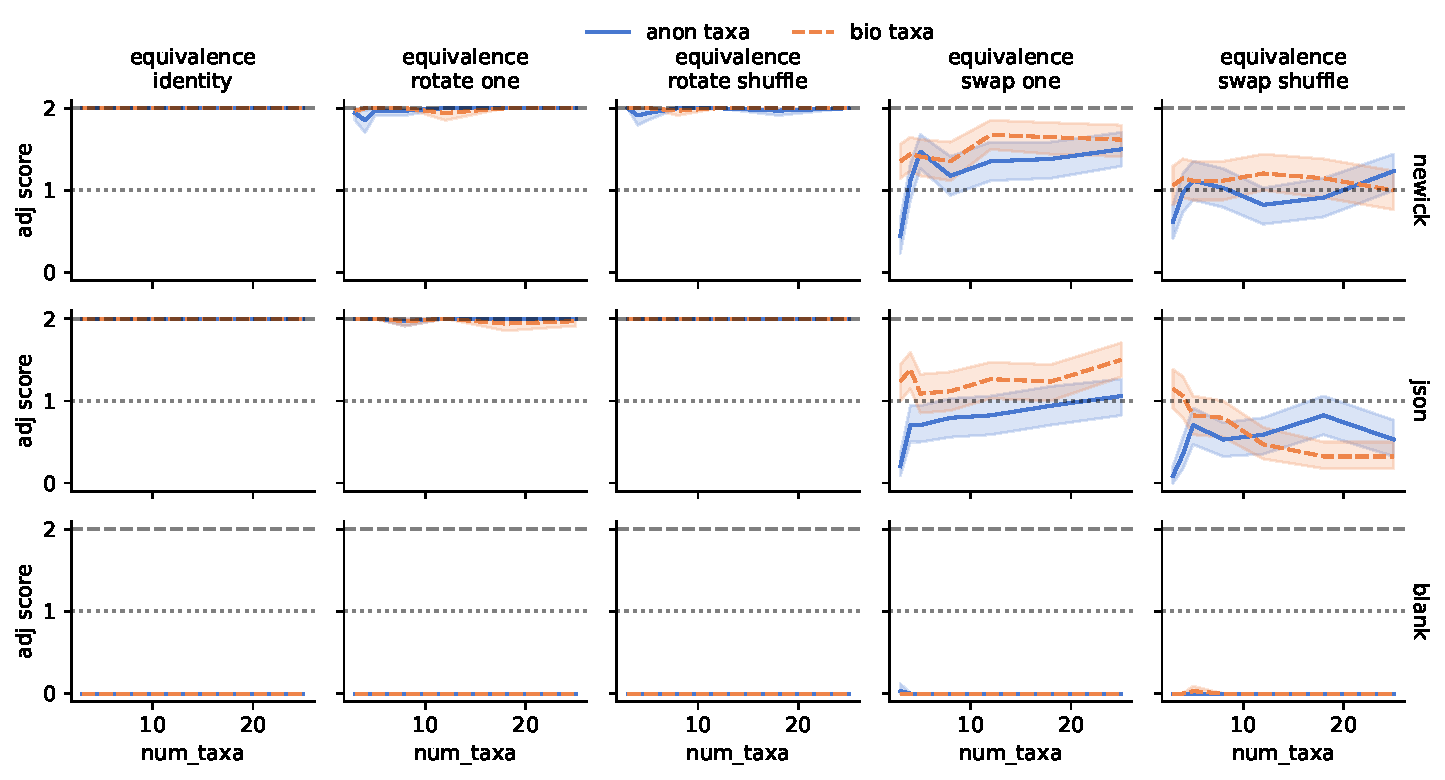
\includegraphics[width=\textwidth, trim={0cm 0cm 1cm 0.7cm}, clip]{binder/binder-2024-11-07-scientific.ipynb/binder/teeplots/2024-11-07-scientific/col=q+hue=tree-source+is_equivalence=True+kind=line+model=gpt-4o+palette=muted+row=tree-repr+style=tree-source+viz=relplot+x=num-taxa+y=adj-score+ext=.pdf}
\end{minipage}%
\begin{minipage}[b]{0.01\textwidth}
\end{minipage}
\begin{minipage}[b]{0.2635\textwidth}
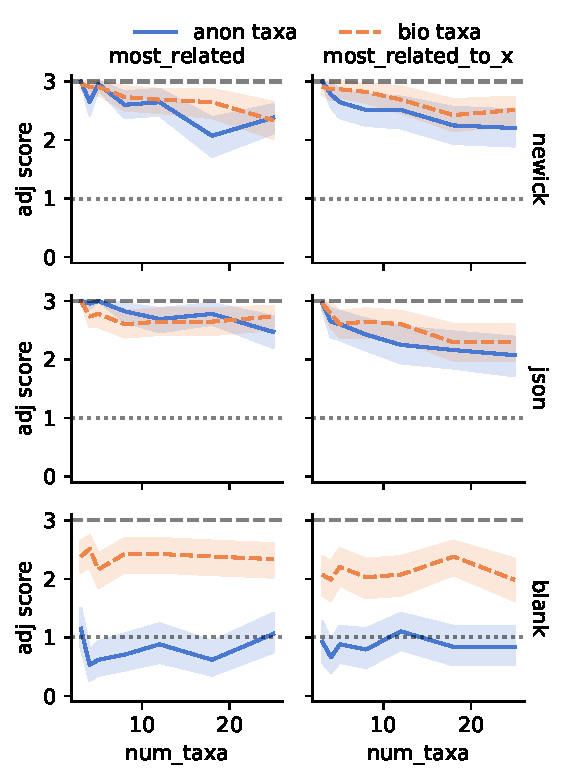
\includegraphics[width=\textwidth, trim={0.65cm 0cm 0cm 0cm}, clip]{binder/binder-2024-11-07-scientific.ipynb/binder/teeplots/2024-11-07-scientific/col=q+hue=tree-source+is_equivalence=False+kind=line+model=gpt-4o+palette=muted+row=tree-repr+style=tree-source+viz=relplot+x=num-taxa+y=adj-score+ext=.pdf}
\end{minipage}
\caption{\footnotesize gpt-4o}
\label{fig:taxatype:gpt-4o}
\end{subfigure}

\begin{subfigure}{\textwidth}
\begin{minipage}[b]{0.7265\textwidth}
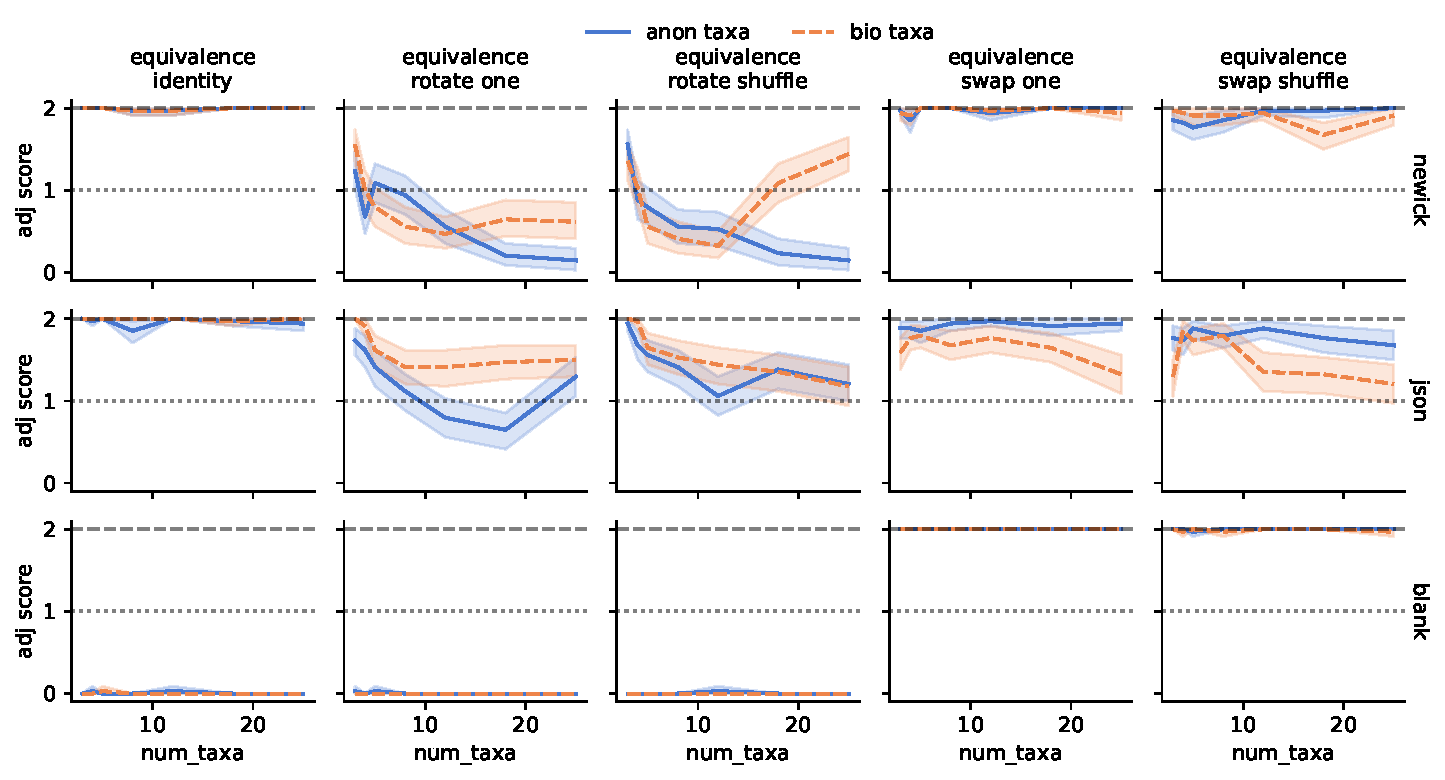
\includegraphics[width=\textwidth, trim={0cm 0cm 1cm 0.7cm}, clip]{binder/binder-2024-11-07-scientific.ipynb/binder/teeplots/2024-11-07-scientific/col=q+hue=tree-source+is_equivalence=True+kind=line+model=gpt-4o-mini+palette=muted+row=tree-repr+style=tree-source+viz=relplot+x=num-taxa+y=adj-score+ext=.pdf}
\end{minipage}%
\begin{minipage}[b]{0.01\textwidth}
\end{minipage}
\begin{minipage}[b]{0.2635\textwidth}
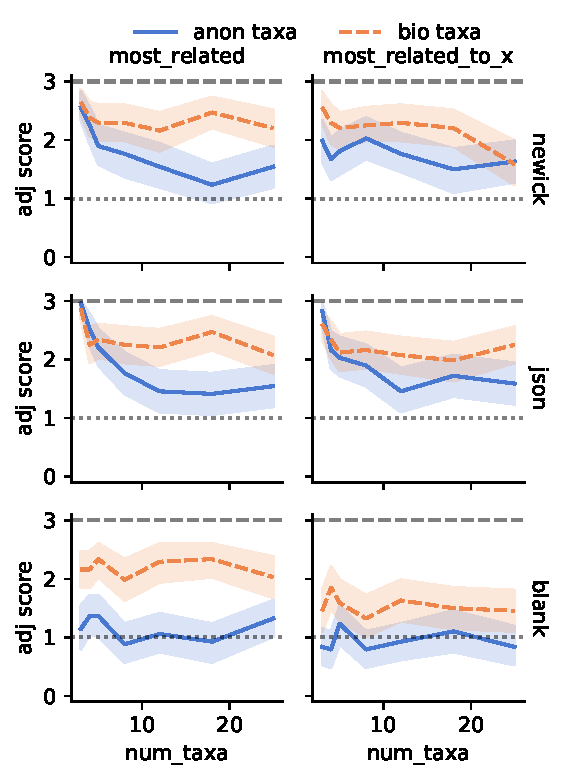
\includegraphics[width=\textwidth, trim={0.65cm 0cm 0cm 0cm}, clip]{binder/binder-2024-11-07-scientific.ipynb/binder/teeplots/2024-11-07-scientific/col=q+hue=tree-source+is_equivalence=False+kind=line+model=gpt-4o-mini+palette=muted+row=tree-repr+style=tree-source+viz=relplot+x=num-taxa+y=adj-score+ext=.pdf}
\end{minipage}
\caption{\footnotesize gpt-4o-mini}
\label{fig:taxatype:gpt-4o-mini}
\end{subfigure}

\caption{
\textbf{Comparison of LLM tree thinking performance for abstract versus species phylogenies.}
\footnotesize
Charts compare tree thinking test scores for prompts constucted using randomly-generated versus biologically-derived phylogenies.
In randomly-generated ``anonymous'' phylogenies, taxa were identified as T0, T1, etc.
``Biological'' phylogenies were subsampled from the Emoji tree of life \citep{mammola2023biodiversity} and taxa were identified via binomial nomenclature (e.g., \textit{Panthera tigris})
Surveyed models include OpenAI GPT-4o (panel \ref{fig:taxatype:gpt-4o}) and OpenAI GPT-4o-mini (panel \ref{fig:taxatype:gpt-4o-mini}).
Adjusted score 1.0, indicated by dotted horizontal line, corresponds to expected correct responses under a random guessing strategy.
Dashed line at top of facets corresponds to best-possible performance, where all responses are correct.
Lattice rows differentiate tree rendering formats: Newick, JSON, or blank (empty string control).
Note, in particular, that under the control ``blank'' tree treatment, biological taxa provide sufficient information to answer the ``most related'' and ``most related to $x$'' questions.
Shaded bands denote bootstrapped 95\% CI, $n=100$.
}
\label{fig:taxatype}

\end{figure*}
